\documentclass{Controle}
\usepackage{multirow}

\begin{document}

\renewcommand{\correction}{oui}

\nom{}

\exercice{Archaeopteryx}
\jesaisfaire{Extraire les caractères d'une espèce d'un texte}
\jesaisfaire{Compléter un tableau de caractères}
\jesais{Je connais quelques caractères (squelette interne, squelette externe, poils, plumes)}

\emph{Archaeopteryx}, qui signifie «~aile antique~», est un genre de
dinosaure à plumes disparu. Comme \emph{Sinocalliopteryx}, on
considère \emph{Archeopteryx} comme un des ancêtres des oiseaux
actuels. Comme eux, il possédait des plumes qu'il utilisait pour le
vol et il avait un squelette interne. En revanche, il ne possédait pas
de bec mais une bouche avec des dents.

\question[]{Complétez le tableau de caractères suivant en mettant une
  croix lorsque le caractère est présent chez l'espèce.}{4}{%
  \newline
  \begin{tabularx}{\linewidth}{|c|*4{Y|}}
    \hline \multirow{2}{*}{\textbf{Caractère}} &
    \multicolumn{4}{c|}{\textbf{Espèce}}\\ \cline{2-5} &
    \emph{Archaeopteryx} & Renard & Canard colvert & Carabe violet \\
    \hline Squelette interne & X & X & X & \\ \hline Squelette externe & & &
    & X \\ \hline Plume & X & & X & \\ \hline Poils & & X & & \\ \hline
  \end{tabularx}
}{%
  \newline
  \begin{tabularx}{\linewidth}{|c|*4{Y|}}
    \hline \multirow{2}{*}{\textbf{Caractère}} &
    \multicolumn{4}{c|}{\textbf{Espèce}}\\ \cline{2-5} &
    \emph{Archaeopteryx} & Renard & Canard colvert & Carabe violet \\
    \hline Squelette interne & & & & \\ \hline Squelette externe & & &
    & X \\ \hline Plume & & & X & \\ \hline Poils & & X & & \\ \hline
  \end{tabularx}
}

\question[]{à partir du tableau de caractères de la question 1,
  complétez la classification en groupes emboîtés ci dessous en
  mettant les noms des groupes suivants :
  \begin{itemize}
  \item Mammifères (possèdent des poils);
  \item Oiseaux (possèdent des plumes);
  \item Vertébrés (possèdent un squelette interne);
  \item Arthropodes (possèdent un squelette externe).
  \end{itemize}
  Attention, chaque boîte, quelle que soit sa taille, ne peut avoir
  qu'un seul nom.}{4}{%
  \newline
  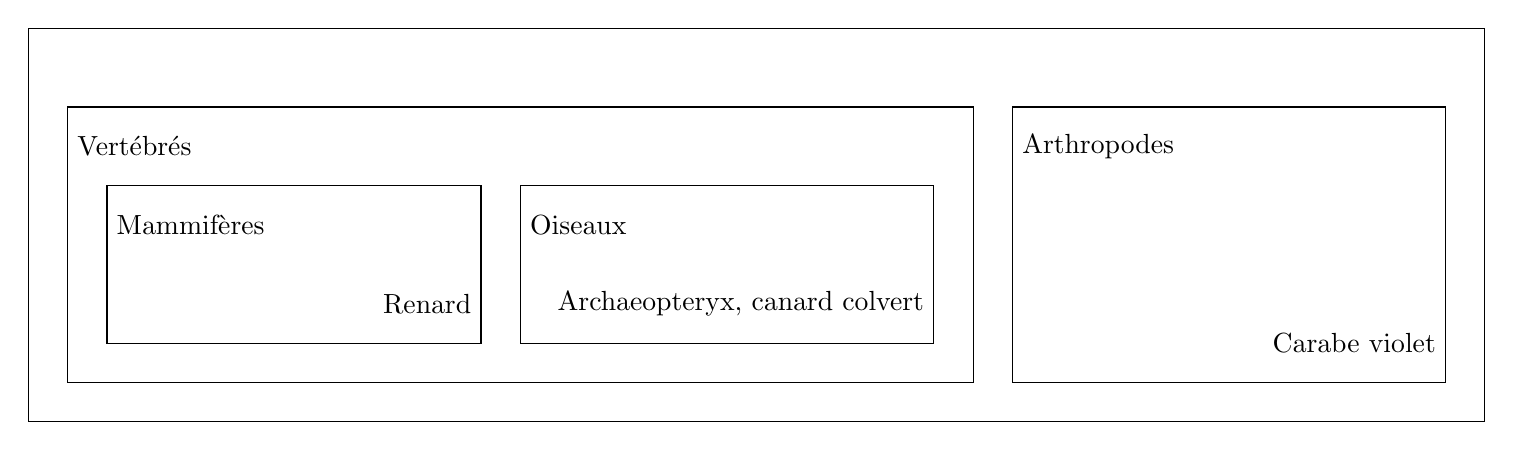
\begin{tikzpicture}
    \draw (0,0) rectangle (18.5,5); %vivant
    \draw (0.5,0.5) rectangle (12,4); %vertébrés
    \draw (12.5,0.5) rectangle (18,4); %arthropodes
    \draw (1,1) rectangle (5.75,3); %mammifères
    \draw (6.25,1) rectangle (11.5,3); %oiseaux
    \node[anchor=west] at (1,2.5) {Mammifères};
    \node[anchor=west] at (6.25,2.5) {Oiseaux};
    \node[anchor=west] at (0.5,3.5) {Vertébrés};
    \node[anchor=west] at (12.5,3.5) {Arthropodes};
    \node[anchor=east] at (5.75,1.5) {Renard};
    \node[anchor=east] at (11.5,1.5) {Archaeopteryx, canard colvert};
    \node[anchor=east] at (18,1) {Carabe violet};
  \end{tikzpicture}}{%
  \newline
  \begin{tikzpicture}
    \draw (0,0) rectangle (18.5,5); \draw (0.5,0.5) rectangle (12,4);
    \draw (12.5,0.5) rectangle (18,4); \draw (1,1) rectangle (5.75,3);
    \draw (6.25,1) rectangle (11.5,3);
  \end{tikzpicture}}

\question[]{Positionnez les quatre espèces du tableau de caractère de
  la question 1 dans les boîtes correspondantes ci-dessus}{4}{}{}
\jesaisfaire{Retrouver le nom des bonnes boîtes dans une classification emboîtée}

\question{La plus grande des boîtes rassemble toutes les espèces qui
  possèdent des cellules. Comment se nomme cette boîte ?}{1}{La plus grande des boîtes se nomme «~Le vivant~»}{}

\jesais{Je sais que la boîte qui regroupe tous les êtres vivants qui possèdent des cellules se nomme «vivant»}
\jesais{Je connais quelques dates de l'histoire de la Terre et de la vie}

\exercice{Histoire de la Terre et de la vie} \question[]{Reliez chacun
  des évènements suivants à la date correspondante.}{7}{%
  \begin{tabularx}{\linewidth}{|X|X|}
    \hline
    La formation de la Terre & 4,56 milliards d'années\\ \hline
    Les premières roches & 4 milliards d'années\\ \hline
    Les premières bactéries & 3,5 milliards d'années\\ \hline
    Les premières cellules avec un noyau & 1,4 milliards d'années\\ \hline
    Les premiers animaux & 600 millions d'années\\ \hline
    La disparition des dinosaures & 65 millions d'années\\ \hline
    L'espèce humaine & moins de un million d'années\\ \hline    
  \end{tabularx}
}{%
  \begin{center}
    \begin{tabular}{lcp{5cm}cl}
      L'espèce humaine & \textbullet & & \textbullet & 65 millions d'années\\
      La formation de la Terre & \textbullet & & \textbullet & 4,56 milliards d'années\\
      Les premières cellules avec un noyau& \textbullet & & \textbullet & 600 millions d'années\\
      La disparition des dinosaures & \textbullet & & \textbullet & 1,4 milliards d'années\\
      Les premières roches & \textbullet & & \textbullet & 3,5 milliards d'années\\
      Les premiers animaux & \textbullet & & \textbullet & Moins de 1 million d'années\\
      Les premières bactéries & \textbullet & & \textbullet & 4 milliards d'années\\
    \end{tabular}
  \end{center}
}

\indic
\end{document}
